\section{Faisal Najib Abdullah}
\subsection{Membaca File SHP}
\begin{enumerate}
	\item 
	\lstinputlisting{src/2/1174042/T2No1.py}
	\begin{figure}[H]
		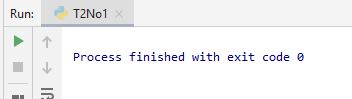
\includegraphics[width=12cm]{figures/1174042/T2No1.JPG}
		\centering
		\caption{Membaca File}
	\end{figure}
	
	\item 
	\lstinputlisting{src/2/1174042/T2No2.py}
	\begin{figure}[H]
		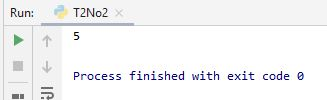
\includegraphics[width=12cm]{figures/1174042/T2No2.JPG}
		\centering
		\caption{Membaca shapeType}
	\end{figure}
	
	\item 
	\lstinputlisting{src/2/1174042/T2No3.py}
	\begin{figure}[H]
		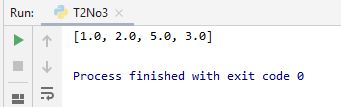
\includegraphics[width=12cm]{figures/1174042/T2No3.JPG}
		\centering
		\caption{Melihat titik titik}
	\end{figure}
	
	\item 
	\lstinputlisting{src/2/1174042/T2No4.py}
	\begin{figure}[H]
		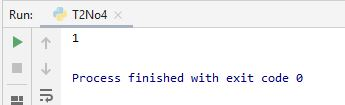
\includegraphics[width=12cm]{figures/1174042/T2No4.JPG}
		\centering
		\caption{Melihat berapa baris}
	\end{figure}
	
	\item 
	\lstinputlisting{src/2/1174042/T2No5.py}
	\begin{figure}[H]
		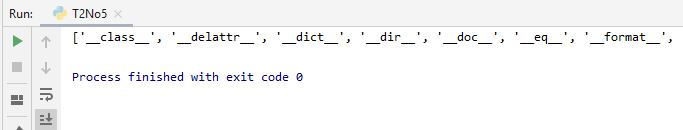
\includegraphics[width=12cm]{figures/1174042/T2No5.JPG}
		\centering
		\caption{Melihat objek}
	\end{figure}
	
	\item 
	\lstinputlisting{src/2/1174042/T2No6.py}
	\begin{figure}[H]
		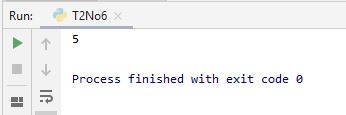
\includegraphics[width=12cm]{figures/1174042/T2No6.JPG}
		\centering
		\caption{Membaca shapeType dengan Shapes}
	\end{figure}
	
	\item 
	\lstinputlisting{src/2/1174042/T2No7.py}
	\begin{figure}[H]
		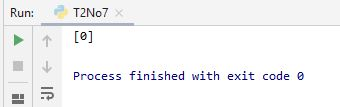
\includegraphics[width=12cm]{figures/1174042/T2No7.JPG}
		\centering
		\caption{Menampilkan indeks titik pertama dari setiap bagian}
	\end{figure}
	
	\item 
	\lstinputlisting{src/2/1174042/T2No8.py}
	\begin{figure}[H]
		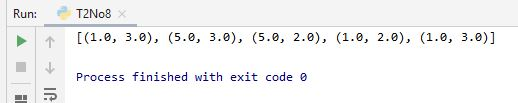
\includegraphics[width=12cm]{figures/1174042/T2No8.JPG}
		\centering
		\caption{Menampilkan titik titik pada bentuk yang dibuat}
	\end{figure}
	
	\item 
	\lstinputlisting{src/2/1174042/T2No9.py}
	\begin{figure}[H]
		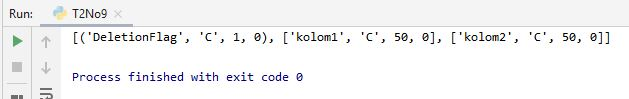
\includegraphics[width=12cm]{figures/1174042/T2No9.JPG}
		\centering
		\caption{Menampilkan kolom dan keterangan pada setiap kolom}
	\end{figure}
	
	\item 
	\lstinputlisting{src/2/1174042/T2No10.py}
	\begin{figure}[H]
		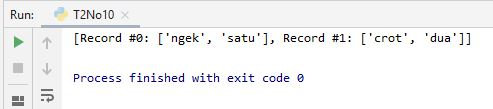
\includegraphics[width=12cm]{figures/1174042/T2No10.JPG}
		\centering
		\caption{Menampilkan isi dari setiap kolom}
	\end{figure}
	
	\item 
	\lstinputlisting{src/2/1174042/T2No11.py}
	\begin{figure}[H]
		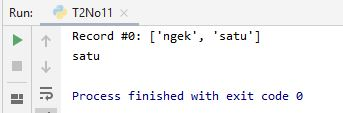
\includegraphics[width=12cm]{figures/1174042/T2No11.JPG}
		\centering
		\caption{Menampilkan isi dari kolom yang ditentukan}
	\end{figure}	
\end{enumerate}

\subsection{Link}
\href{https://youtu.be/mozFVwqvabo}{Youtube}